\section{Architecture}
\label{sec:arch}
The most appealing thing about the proposed compositional architecture is that
it makes implementing a server very easy. If you can construct a data-flow diagram 
representing the conversion of a request into a response, then this diagram
can be directly translated into a program.

In this Chapter I introduce a few example web-servers and their conceptual
design using the proposed architecture. I also introduce a wrapper 
solution used for caching and load balancing.
Finally I compare these designs to the set up of equivalent Apache servers.

\subsection{Hello World!}
\label{sec:helloWorld}
The simplest example is a Hello world! server. This server replies with a 
Hello world! message to all requests and can be represented by the diagram
in Figure \ref{fig:helloWorld}.

\begin{figure}[h]
\centering
\begin{tikzpicture}[node distance = 2cm, auto]
    % Nodes
    \node [listener] (listener) {Listener};
    \node [component, right of=listener, text width=6em,, node distance=4cm] (hello) {Hello World Component};
    \node [writer, right of=hello, node distance=4cm] (writer) {String Writer};
    % Edges
    \path [line] (listener) -- (hello);
    \path [line] (hello) -- (writer);
\end{tikzpicture}
\caption[scale=1.0]{Hello world! server architecture.}
\label{fig:helloWorld}
\end{figure}

The \texttt{Listener} represents the 
part of the program that gets requests and feeds them to the network.
The \texttt{Hello World Component} inputs a client request from its input channel
and outputs the request together with the Hello World! string that should be 
used as a response to its output channel.
The \texttt{String Writer} writes the text response back to the client.

This is a good example of the basic components of the suggested framework.
We can call the three main parts the \texttt{Listener}, \texttt{Processor} 
and \texttt{Writer}, where
the \texttt{Listener} catches the incoming requests and feeds them into the network,
the \texttt{Processor} processes them and the \texttt{Writer} writes the generated result 
back to the client. That is \texttt{Listener} is the start and \texttt{Writer}
is the end of the server pipeline.

\subsection{File Server}
\label{sec:fileServer}
Architecture of a simple file server follows the architecture of the Hello world!
server introduced above. It consists of a \texttt{Listener}, which catches the requests,
\texttt{File Getter}, what is a function that gets the requested file (that is it
constructs the absolute path to the requested file and loads it into the memory) 
and finally there is a \texttt{File Writer}, which
writes the file to the client. The architecture is shown in Figure \ref{fig:fileServer}.
\begin{figure}[h]
\centering
\begin{tikzpicture}[node distance = 2cm, auto]
    % Nodes
    \node [listener] (listener) {Listener};
    \node [component, right of=listener, node distance=4cm] (getter) {File Getter};
    \node [writer, right of=getter, node distance=4cm] (writer) {File Writer};
    % Edges
    \path [line] (listener) -- (getter);
    \path [line] (getter) -- (writer);
\end{tikzpicture}
\caption[scale=1.0]{File server.}
\label{fig:fileServer}
\end{figure}

If we want to compress some subset of files, we can just add a \texttt{Splitter}
that sends files that are supposed to be compressed to a \texttt{Gzip Writer}, which
compresses the file and writes the result to the client. The rest of the files
will be passed to the standard \texttt{File Writer}. This architecture is shown in
Figure \ref{fig:fileServer2}.

\begin{figure}[h]
\centering
\begin{tikzpicture}[node distance = 2cm, auto]
    % Nodes
    \node [listener] (listener) {Listener};
    \node [component, right of=listener, node distance=3cm] (getter) {File Getter};
    \node [component, right of=getter, node distance=3cm] (splitter) {Splitter};
    \node [writer, right of=splitter, node distance=3cm] (fwriter) {File Writer};
    \node [writer, below of=fwriter] (gwriter) {Gzip Writer};
    % Edges
    \path [line] (listener) -- (getter);
    \path [line] (getter) -- (splitter);
    \path [line] (splitter) -- (fwriter);
    \path [line] (splitter) |- (gwriter);
\end{tikzpicture}
\caption[scale=1.0]{File server with compression.}
\label{fig:fileServer2}
\end{figure}

\subsection{Caching}
Suppose we have a worker component, which performs some expensive computation
and that we want to cache its output.
Using the proposed architecture we can just wrap the worker in a caching layer.
That is we only run the worker component if we don't have the result
in the cache, otherwise we just return the stored result. 
This design is show in Figure \ref{fig:caching}.

\begin{figure}[h]
\centering
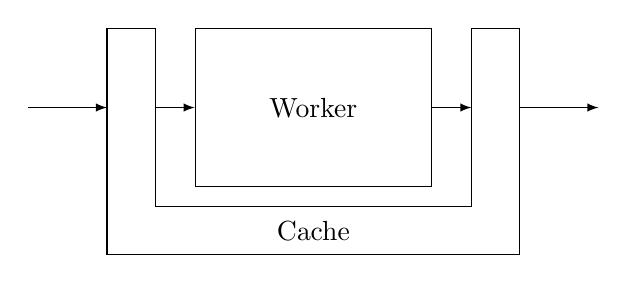
\begin{tikzpicture}[
    workerWidth/.style={minimum width=3cm},
    workerHeight/.style={minimum height=2cm},
    UWidth/.style={minimum width=0.6cm},
    every node/.style={
        text centered,
        }
        ]
    \node[workerWidth, workerHeight, draw] (worker) at (0, 0) {Worker};

    \node[anchor=north, minimum height=0.6cm, workerWidth, yshift=-0.25cm] (cache) at (worker.south) {Cache};

    \node[anchor=east, workerHeight, UWidth, xshift=-0.5cm] (left) at (worker.west) {};
    \node[anchor=west, workerHeight, UWidth, xshift=0.5cm] (right) at (worker.east) {};

    \draw (left.north west) -- (left.west |- cache.south) -- (right.east |- cache.south) -- (right.north east) -- (right.north west) -- (right.west |- cache.north) -- (left.east |- cache.north) -- (left.north east) -- cycle;

    \draw[<-, >={latex}] (left.west) -- ++(-1, 0);
    \draw[->, >={latex}] (left.east) -- (worker.west);
    \draw[->, >={latex}] (worker.east) -- (right.west);
    \draw[->, >={latex}] (right.east) -- ++(1, 0);
\end{tikzpicture}\caption[scale=1.0]{Caching output of a worker component.}
\label{fig:caching}
\end{figure}

\subsection{Load Balancing}
If there is a lot of traffic in a certain part of the network we can
increase the throughput there
by creating multiple instances of the components in this part of 
the pipeline. The incoming request can then be passed to the component that is 
ready first. When the load in a given part of the pipeline decreases,
we can shut down the created components.

The benefit of the proposed architecture is that, we can do these adjustments
in runtime.
That is, based on current number of requests going through a certain part of 
the network we can decide to add or remove parts of the pipeline. This does not
have to be only adding components locally.
If we use channels over network then
we can connect to other servers and distribute the workload among them.
Hence we can start or shut down other servers based on the current traffic.
See Figure \ref{fig:loadBalancing}.

\begin{figure}[h]
\centering
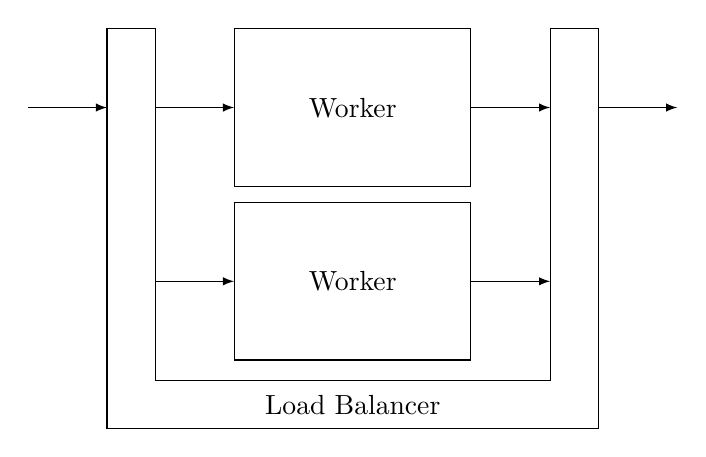
\begin{tikzpicture}[
    workerWidth/.style={minimum width=3cm},
    workerHeight/.style={minimum height=2cm},
    UWidth/.style={minimum width=0.6cm},
    every node/.style={
        text centered,
        }
        ]
    \node[workerWidth, workerHeight, draw] (worker) at (0, 0) {Worker};
    \node[workerWidth, workerHeight, yshift=-1.2cm, draw] (worker2) at (worker.south) {Worker};

    \node[anchor=north, minimum height=0.6cm, workerWidth, yshift=-0.25cm] (cache) at (worker2.south) {Load Balancer};

    \node[anchor=east, workerHeight, UWidth, xshift=-1cm] (left) at (worker.west) {};
    \node[anchor=west, workerHeight, UWidth, xshift=1cm] (right) at (worker.east) {};
    \node[anchor=east, workerHeight, UWidth, xshift=-1cm] (left2) at (worker2.west) {};
    \node[anchor=west, workerHeight, UWidth, xshift=1cm] (right2) at (worker2.east) {};

    \draw (left.north west) -- (left.west |- cache.south) -- (right.east |- cache.south) -- (right.north east) -- (right.north west) -- (right.west |- cache.north) -- (left.east |- cache.north) -- (left.north east) -- cycle;

    \draw[<-, >={latex}] (left.west) -- ++(-1, 0);
    \draw[->, >={latex}] (left.east) -- (worker.west);
    \draw[->, >={latex}] (worker.east) -- (right.west);
    \draw[->, >={latex}] (left2.east) -- (worker2.west);
    \draw[->, >={latex}] (worker2.east) -- (right2.west);
    \draw[->, >={latex}] (right.east) -- ++(1, 0);
\end{tikzpicture}\caption[scale=1.0]{
    Managing load in a given part of the network.
    One of the workers can be shut down or more workers can be added.
}
\label{fig:loadBalancing}
\end{figure}

\subsection{Comparison to Apache server configuration}
As noted before configuring an Apache serer can prove to be quite difficult.
Below in Figure \ref{fig:apache} is shown a part of a simple file server
configuration.
\begin{figure}[h]
\centering
\begin{lstlisting}[numbers=left]
Alias /project /path/to/project/

<Directory "/path/to/project/">
    Options Indexes
    AllowOverride None
    Order allow,deny
    Allow from localhost
    Require all granted
    AddOutputFilter DEFLATE py
</Directory>
\end{lstlisting}
\caption[scale=1.0]{Part of Apache configuration file for a file server.}
\label{fig:apache}
\end{figure}
% TODO: explain the whole configuration
The first line in the above configuration specifies that accessing URL 
path "/project" should point to the "/path/to/project/" directory.
Lines 3 to 10 specify who and how can access this directory.
The option \texttt{Options Indexes} indicates that if a client tries
to access a directory, then the server should list its contents.

\texttt{AllowOverride None} disables access to other directives when 
a file in the specified folder is accessed. Lines 6 to 8 specify that
anyone can access the directory. Finally, option 
\texttt{AddOutputFilter DEFLATE py} tells the server to compress
all python files, that is all files whose name ends with '.py'.

At first this does not look like a difficult configuration. However, 
one might argue that it is not as clear as the architecture proposed above,
as we are mixing different aspects of the server in one place.
The main issue is that configuring more complex servers gets much more 
difficult very quickly. Furthermore if we want to serve dynamic content
we might need to use scripts written in other languages such as perl or python.

\subsection{Summary}
In this Chapter I described the conceptual architecture of the proposed
toolkit on a few simple examples. Then I showed configuration of a simple
Apache file server and contrasted this with my proposed architecture.
The next Chapter introduces the basic elements of my implementation.
